\documentclass{beamer}
\graphicspath{ {../images/} }
\usepackage[export]{adjustbox}

\title{Text to SQL Generation}
\author{Jake Waffle}
\date{2023}

\begin{document}

\frame{\titlepage}

\begin{frame}
\frametitle{Swagger UI}

\adjincludegraphics[trim={{.12\width} {0.3\height} {.5\width} {0.07\height}},clip,scale=0.4]{swagger-ui-example3.png}

\end{frame}

\begin{frame}
\frametitle{Swagger UI}

\adjincludegraphics[trim={{.18\width} {0.11\height} {.1\width} {0.24\height}},clip,scale=0.32]{swagger-ui-example4.png}

\end{frame}


\begin{frame}
\frametitle{Architecture}

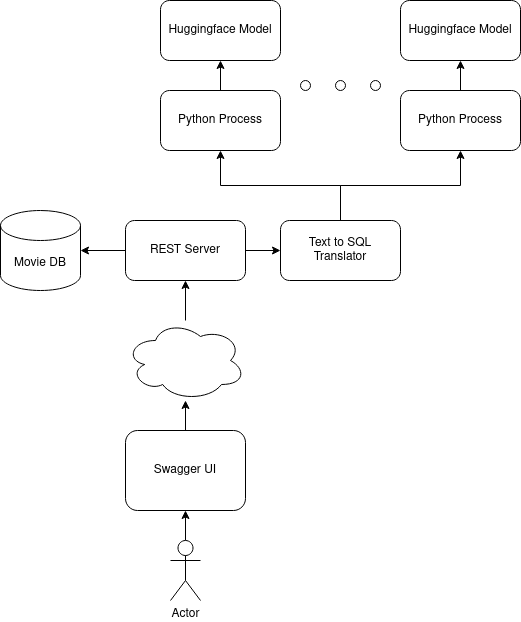
\includegraphics[scale=0.4]{demo-architecture.drawio.png}

\end{frame}

\begin{frame}
\frametitle{Transformer}

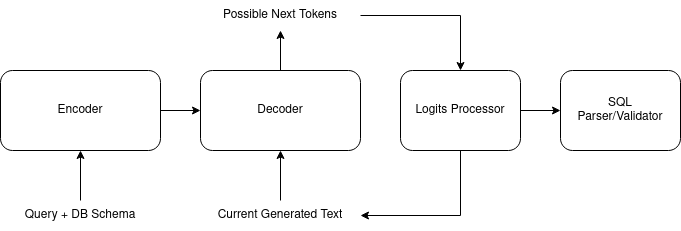
\includegraphics[scale=0.45]{t5-transformer.drawio.png}

\end{frame}

\begin{frame}
\frametitle{Why}

\begin{itemize}[<+->]
  \item Manually supporting filters is maintenance heavy on the frontend/backend
  \item Users don't like learning query languages like OData and reading documentation
  \item The model used isn't trained against a specific database schema
\end{itemize}

\end{frame}

\begin{frame}
\frametitle{Pitfalls}

\begin{itemize}[<+->]
  \item PEG parsers aren't well suited for incrementally validating generated text in the logits processor
  \item Text generation support in libraries is generally immature
  \item Python's GIL makes Huggingface's `model.generate()` unable to be used in multiple threads
\end{itemize}

\end{frame}

\begin{frame}
\frametitle{Evaluation}

\begin{itemize}[<+->]
  \item Spider text to SQL dataset
  \item Content overlap
\end{itemize}

\end{frame}


\end{document}
